\begin{exercise}
Υπολογίστε στο επίπεδο τον μετασχηματισμό στροφής γωνία $\theta = \cfrac{\pi}{3}$ γύρω από το σημείο $P = (4,1)$

Στην συνέχεια, γράψτε ένα script σε \texttt{Julia} όπου θα υπολογίζει τον παραπάνω πίνακα μετασχηματισμού μέσω πολλαπλασιασμών των βασικών μετασχηματισμών και εφαρμόστε τον, στο παρακάτω σχήμα  σχεδιάζοντας στο ίδιο γράφημα και το αρχικό και το μετασχηματισμένο.

\begin{figure}[hbt]
  \begin{center}
	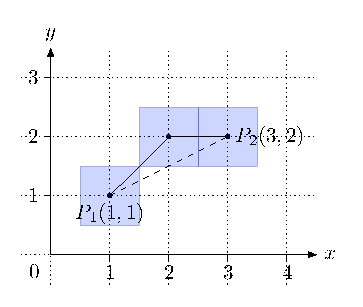
\includegraphics[scale=1]{Chapter1/Exercises/ex17/graph1.pdf}
  \end{center}
%  \caption{Παράσταση ζητούμενων ευθυγ\textcolor{red}{what}ράμμων τμημάτων}
\end{figure}

\end{exercise}